\documentclass[digital, oneside, table, nolot, nolof]{fithesis3}

%% The following section sets up the locales used in the thesis.
\usepackage[resetfonts]{cmap}
\usepackage[T1]{fontenc}
\usepackage[main=czech, english]{babel}

%% The following section sets up the metadata of the thesis.
\thesissetup{
    date          = \the\year/\the\month/\the\day,
    university    = mu,
    faculty       = fi,
    type          = bc,
    author        = Jan Horáček,
    gender        = m,
    advisor       = Zdeněk Matěj,
    title         = {Systém automatické kalibrace modelového železničního vozidla},
    TeXtitle      = {Systém automatické kalibrace modelového železničního vozidla},
    keywords      = {kalibrace, dcc, vlak, model, senzor},
    TeXkeywords   = {kalibrace, dcc, vlak, model, senzor},
    abstract      = {Tady bude abstrakt.},
    thanks        = {Děkuji Losu Karlosovi za skvělý metaprogram!},
    bib           = bibliography.bib,
}
\usepackage{makeidx}      %% The `makeidx` package contains
\makeindex                %% helper commands for index typesetting.
%% These additional packages are used within the document:
\usepackage{paralist} %% Compact list environments
\usepackage{amsmath}  %% Mathematics
\usepackage{amsthm}
\usepackage{amsfonts}
\usepackage{url}      %% Hyperlinks
\usepackage{listings} %% Source code highlighting
\lstset{
  basicstyle      = \ttfamily,%
  identifierstyle = \color{black},%
  keywordstyle    = \color{blue},%
  keywordstyle    = {[2]\color{cyan}},%
  keywordstyle    = {[3]\color{olive}},%
  stringstyle     = \color{teal},%
  commentstyle    = \itshape\color{magenta}}
\usepackage{floatrow} %% Putting captions above tables
\floatsetup[table]{capposition=top}
\begin{document}

\chapter*{Úvod}
\addcontentsline{toc}{chapter}{Úvod}

Říká se, že závěrečné práce jsou vyvrcholením studia a tak jsem se
rozhodl jednu také napsat. Pokud vše půjde podle plánu, odnesu si
na konci semestru diplom. Držte mi palce!

\chapter{Úvod} \label{chap:uvod}
Současná modelová kolejiště již dávno nejsou jen hračkou malých dětí
a jejich rodičů. Jsou to plnohodnotné modely, na kterých se dispečeři skutečné
železnice učí řídit dopravu a~které slouží pro výuků oborů automatizace.
Kolejiště jsou vybavena robustní a~spolehlivou zabezpečovací technikou
podobnou té, která se v~současnosti používá na skutečné železnici.

S~růstem rozměrů kolejišť a~cen modelů vzniká nutnost procesy řízení
automatizovat, předejít chybám způsobeným lidským faktorem a~řízení kolejiště
obecně zefektivnit. Cílem této práce je pomocí automatizace procesu kalibrace
modelového železničního vozidla přispět právě ke zvýšení bezpečnosti
a~spolehlivosti provozu.

Autor rozebere možnosti řešení problému automatické kalibrace, ukáže, proč jsou
současná řešení nevhodná a~nakonec navrhne (1) hardware, (2) firmware a~(3)
software, kterými uvedený problém řeší. Autor demonstruje výstupy této práce
v~praxi a~ukáže její reálný přínos.

Tuto práci je tematicky možné zařadit jednak do kategorie \textit{proof of
concept}, druhak však i~do kategorie práce \textit{aplikační}. Jejím primárním
cílem totiž je vytvořit reálné řešení reálného problému v~oblasti automatizace,
který doteď ještě nikdo neřešil. Konkrétně se práce zaměřuje na automatizaci
řízení dopravy na modelovém kolejišti. Cílem této práce je navrhnout kvalitní
řešení od hardwaru, přes firmware až po software.

Pro přesnou formulaci problému automatické kalibrace železničního vozidla je
nutné pochopit kontext této práce, o~kterém pojednává tato kapitola.

\section{Modelová kolejiště}
\label{sec:mod-kol}

Modelové kolejiště je model železniční tratě, typicky zmenšený
v~některém ze standardních měřítek, např. v~měřítku \uv{TT} (1:120) či \uv{H0}
(1:87). Vedle typického \uv{hobby} využití kolejiště často slouží jako dopravní
trenažéry pro výuku zabezpečovacích zařízení železnice či dalších aspektů
využívaných na skutečné železnici. Nejen v~těchto případech vzniká potřeba
kolejiště ovládat \textit{zabezpečovacím zařízením}. Typickým příkladem
současného zabezpečovacího zařízení na skutečné železnici je
\textit{elektronické stavědlo} spolu s~grafickou nadstavbou
\textit{JOP} (\textit{Jednotné obslužné pracoviště}), která umožňuje řízení
stavědla přes počítač.

Obdobný systém je využíván také v~\textit{Klubu modelářů železnic Brno I}.
V~tomto klubu je nasazen systém řízení kolejišť zvaný \textit{hJOP}
\cite{hjop:web}, který je klonem JOP upraveným pro potřeby řízení modelu. Jeho
primárním cílem je řídit jízdu vlaku a~omezením lidského faktoru předejít
možným kolizím.

\section{Současné trendy v~řízení kolejiště}
\label{sec:trendy}

K~řízení modelových kolejišť je v~současné době napříč zeměmi využívána celá
řada dostupných SW. Typickými příklady jsou například \textit{JMRI}
\cite{jmri:web}, \textit{TrainController} \cite{traincontroller:web}
nebo český SW \textit{modelJOP} \cite{modeljop:web}.

Výše zmíněné aplikace potřebují komunikovat s~hardwarovými prvky kolejiště.
Nejdůležitějším z~těchto prvků je digitální centrála DCC. Digitální centrála je
obecný pojem, konkrétními instancemi od jednotlivých výrobců jsou pak např.
\textit{Z21} \cite{z21:web}, \textit{NanoX} \cite{nanox:web} nebo třeba
\textit{Intellibox} \cite{intellibox:web}. Centrála nejčastěji komunikuje
s~počítačem pomocí sběrnice \textit{RS232 over USB}. Jejím hlavním úkolem je
vytvářet \textit{digitální signál DCC} \cite{nmra:dcc:ele}, který moduluje do
kolejí.

Lokomotiva stojící na kolejích tento signál dekóduje pomocí spe\-ciál\-ní
součástky -- tzv. \textit{dekodéru DCC} -- a~podle přijatých dat poveluje
periferie lokomotivy: motor, světla, nebo třeba zvuk vydávaný vestavěným
reproduktorem. Modulovaný výkonový signál v~kolejích je zároveň využíván jako
(1) nosič informace pro dekodéry a~(2) po usměrnění jako napájecí napětí pro
periferie, včetně výkonově nejnáročnější periferie -- motoru. Dekodér
v~podstatě obsahuje jen jednoduchý mikrokontrolér a~několik výkonových prvků.
Jeho typická velikost je v~řádu malých jednotek cm$^2$, takže je skutečně malý.

Každý dekodér má svoji adresu v~rozsahu $1$--$9999$. Počítač pak může vydat příkaz
pro řízení lokomotivy, např.: \textit{\uv{lokomotivo s~adresou 562, jeď směrem
vpřed rychlostí 15!}}

Každý dekodér si ukládá svá konfigurační data do volatilní paměti formou tzv.
\textit{CV} (\textit{Configuration Value}). \textit{CV} je jedna konfigurační
jednotka s~rozsahem hodnot 1~byte ($0$--$255$). Každé \textit{CV} má svoje číslo
(typicky $1$--$1023$). Výrobce dekodéru (potažmo standardizační organizace) pak
definuje význam jednotlivých CV. Například CV $\#17$ a~$\#18$ jsou vyhrazeny
k~uložení adresy dekodéru \cite{zimo:cvs}.

\section{Synchronizace rychlosti vozidel}
\label{sec:sync-rych}

Rychlost lokomotivy typicky bývá přirozené číslo v~rozsahu $0$--$28$. Tato
hodnota se označuje jako tzv. \textit{jízdní stupeň}.

Protože každá lokomotiva obsahuje jiné mechanické prvky (převody, motor),
odpovídá stejnému jízdnímu stupni u~dvou různých nezkalibrovaných hnacích
vozidel různá rychlost. Ukazuje se, že při řízení kolejiště je vhodné, aby (1)
stejnému jízdnímu stupni u~všech hnacích vozidel na kolejišti odpovídala stejná
rychlost a~aby (2) byl jízdní stupeň pevně spárovaný s~reálnou rychlosti
vozidla přepočtenou dle měřítka.

Synchronizací rychlosti vozidel myslíme právě splnění těchto dvou vlastností
pro všechny lokomotivy na kolejišti. Proces synchronizace rychlostí je součásti
procesu \textit{kalibrace lokomotivy}.

Motivací pro tyto kroky je především to, abychom dosáhli modelové věrnosti
a~aby se vozidlo po přepočtu pohybovalo \textit{modelovou rychlostí}. Je také
nutné dbát na provozní parametry kolejiště, které umožňují průjezd některými
částmi kolejiště jen omezenou rychlostí. Při překročení této rychlosti by pak
mohlo dojít k~vykolejení, což je samozřejmě nežádoucí.

Dalším důvodem pro synchronizaci je vytvoření předvídatelného prostředí pro
obsluhu. Obsluha má často k~dispozici ovladač pro řízení rychlosti jízdy
vozidla v~ručním režimu. Autor této práce považuje za velice užitečné, aby
platilo, že otočení trimru ovladače o~daný úhel způsobí u~všech vozidel pohyb
stejnou rychlostí (úhel otočení trimru ovladače odpovídá jízdnímu stupni).

Třetím důvodem k~synchronizaci rychlostí vozidel je umožnění přípřeží a~postrků
-- tj.  situací, kdy v~jednom vlaku jede více lokomotiv. Tyto lokomotivy se
musí pohybovat stejnou rychlostí, jinak hrozí vykolejení vlaku.

\subsection{Současné řešení problému}

Současné řídicí programy problém synchronizace rychlostí typicky řeší tak, že
si u~každého hnacího vozidla ukládají tabulku \textit{jízdní stupeň: rychlost}.
Když tyto programy chtějí, aby dvě lokomotivy jely stejnou rychlostí, vyhledají
příslušné jízdní stupně a~do centrály (v~obecném případě) odešlou pro každou
lokomotivu jiný jízdní stupeň.

Provozu lokomotivy na kolejišti tak předchází buď

\begin{compactitem}
	\item ruční zadání této tabulky, nebo
	\item automatické měření rychlosti lokomotivy.
\end{compactitem}

Je však nutné podotknout, že toto řešení neuspokojuje naše požadavky pro
ruční řízení jízdy hnacího vozidla, protože tabulka rychlostí je uložena
pouze v~řídicím SW, s~kterým nebývají ovladače propojeny, takže nemohou tabulku
využít. Stejnému úhlu otočení trimru ovladače tak zpravidla odpovídají různé
rychlosti u~různých lokomotiv, přípřeže a~postrky jsou prakticky nemožné.

\subsection{Řešení problému v~hJOP}

Alternativním řešením problému synchronizace rychlostí je způsob, který
v~současné době využívá SW hJOP. Tato práce cílí právě na onen alternativní
způsob řešení kalibrace. Jeho výhoda je v~tom, že řeší synchronizaci
rychlostí i~pro ruční ovladače.

V~každém lokomotivním dekodéru je možno pro každý z~28 jízdních stupňů nastavit
konkrétní otáčky motoru. SW hJOP předpokládá, že uživatel provede před
provozem hnacího vozidla tzv. \textit{kalibraci}, tj. přiřazení otáček motoru
každému rychlostnímu stupni každého vozidla tak, aby bylo splněno, že konkrétní
jízdní stupeň odpovídá u~všech vozidel stejné rychlosti.

Příklad: u~všech lokomotiv platí, že jízdní stupeň $15$ odpovídá rychlosti $40\
km/h$.

Dalšími výhodami tohoto řešení jsou:

\begin{compactenum}
	\item odpadnutí nutnosti udržovat si u~každého vozidla v~SW kalibrační
	tabulku a
	\item instantní přenos tabulky mezi kolejišti, když je přenesena
	lokomotiva (to proto, že tabulka je jednoduše fyzicky uložená v~lokomotivě,
	a tudíž logicky cestuje s~ní).
\end{compactenum}

Nevýhodou tohoto přístupu je, že je nutné provést netriviální proces kalibrace.
V~současné době tento proces zahrnuje ježdění s~lokomotivou na měřicím okruhu,
měření její rychlosti a~ruční nastavování kalibrační tabulky.

Cílem této práce je tento proces automatizovat.

\section{Synchronizace brzdných křivek vozidel}
\label{sec:sync-krivky}

Možná ještě fundamentálnějším problémem, než synchronizace rychlostí, je
synchronizace délky dojezdu z~určité fixní rychlosti napříč různými vozidly.
Lokomotivní dekodér má pro tento účel vyhrazeno CV $\#4$ \cite{zimo:cvs}, které
definuje dobu brzdění. Při nenulové hodnotě tohoto CV tak dekodér po obdržení
příkazu \uv{stůj} nezastaví ihned, ale postupně zpomaluje.

Tento parametr je naprosto klíčový, ovládací SW totiž typicky vyžaduje, aby dané
vozidlo zastavilo na konkrétní pozici (před návěstidlem, u~nástupiště, ...).
Současné ovládací aplikace problém synchronizace dojezdů řeší typicky tak, že si
dojezd změří a~dále s~ním kalkulují v~dalších výpočtech. Například program
\textit{TrainController} \cite{traincontroller:web} dokonce při brzdění
posílá dekodéru postupně povely \uv{jeď stupněm 12}, \uv{jeď stupněm 10},
\uv{jeď stupněm 5}, ..., takže se efekt brzdné křivky prakticky eliminuje.

Autor této práce považuje toto řešení za nešťastné, neboť
\begin{compactenum}
\item se zásadně zvyšuje datový tok mezi SW a~centrálou,
\item je třeba si u~každé lokomotivy udržovat další data,
\item po převzetí lokomotivy na ruční ovladač se každá lokomotiva chová jinak a
\item při jízdě přes ruční ovladač jsou typicky dojezdy tak malé, že lokomotiva
      brzdí nemodelově rychle.
\end{compactenum}

Proto byl při tvorbě SW hJOP zvolen alternativní přístup. Je striktně
definováno, že \textit{každá lokomotiva musí z~rychlosti 40 km/h zastavit na
$30$--$35\ cm$}.\footnote{Tato hodnota se liší pro jednotlivá měřítka,
$30$--$35\ cm$ je standard pro měřítko TT 1:120.} Do této vzdálenosti od
kýženého bodu zastavení jsou do kolejiště fyzicky montovány senzory. Po
projetí vozidla senzorem pošle hJOP povel \uv{lokomotivo s~adresou 1254, stůj!},
lokomotiva začne plynule brzdit a~do přesně dané vzdálenosti zastaví. A~to vše
modelově plynule.

Kalibrace dojezdů zajišťuje to, že hnací vozidlo nikdy nepřejede návěstidlo nebo
nenajede do špatně postavené výměny. Je proto ještě důležitější než kalibrace
rychlosti.\footnote{Kdyby uživatel zkalibroval lokomotivu tak, aby jezdila
hodně rychle, ale pořád dodržel $30$--$35cm$ brzdnou vzdálenost z~rychlostního
stupně 15 (ten odpovídá dle standardu KMŽ $40\ km/h$), lokomotiva nikdy nevjede,
kam nemá.}

Součástí procesu kalibrace by tedy měla být také synchronizace brzdných křivek.

\section{Cíl práce}
\label{sec:cil}

Cílem této práce je automatizovat proces kalibrace lokomotivy.

Nejprve je nutné navrhnout metodu pro měření rychlosti hnacího vozidla
a~zabezpečit přenos naměřených dat do řídicího PC. Poté je nutné navrhnout SW,
který na nákladě změřené rychlosti nastaví kalibrační tabulky hnacího vozidla.

Výstupem této práce je řešení, které umožní proces kalibrace především
automatizovat, což povede k~ušetření lidských kapacit. Dále umožní proces
kalibrace zrychlit, což přispěje k~minimalizaci režijního času spojeného
s~provozem kolejiště, a~zároveň proces kalibrace zpřesnit, což povede ke
zvýšení spolehlivosti provozu na kolejišti.


\chapter{Požadavky na řešení} \label{chap:pozadavky}
Pro návrh vhodného řešení procesu automatické kalibrace je nutné formulovat
požadavky kladené na toto řešení. Základní požadavky seřazené od
nejdůležitějšího jsou:

\begin{compactenum}
	\item snadné použití pro koncového uživatele, snadná instalace,
	\item možnost použít řešení pro libovolné modelové měřítko,
	\item maximalizace automatizace a~minimalizace nutné spolupráce s~uživatelem,
	\item urychlení procesu kalibrace,
	\item možnost provést dokalibrování za skutečného provozu,
	\item přehledné verzování projektu, čistý a~přehledný kód, využití otevřených
	technologií.
\end{compactenum}

První bod vyplývá z~faktu, že proces kalibrace bude často spouštěn laickou obsluhou
kolejiště. Proto bude kladen důraz na očekávatelné chování grafického
rozhraní a~jednoduchost práce se samotným měřicím hardwarem. Řešení bude také
navrženo tak, aby využívalo běžně dostupné technologie, se kterými jsou
uživatelé zvyklí pracovat.

Stejně jako jinde ve světě, tak i~v~brněnském Klubu je provozováno více
modelových měřítek, autor se vynasnaží navrhnout řešení tak, aby bylo nezávislé
na měřítku.

Za okomentování dále stojí bod (5). Po zakoupení nového vozidla se
typicky provádí jeho kalibrace, vozidlo je následně začleněno do provozu, kde
jezdí i~několik let. Fyzikální realita světa je bohužel neúprosná --
ve vozidle dochází k~mechanickému opotřebení prvků, zaběhnutí pohyblivých
částí po určité době provozu a~ke změně mechanických parametrů vozidla
v~závislosti na teplotě. Důsledkem těchto skutečností je, že kalibrace vozidla
po určité době ztrácí přesnost. Vychýlení typicky není zásadní, ale mnohdy
znatelné.

Proto je vhodné navrhnout kalibrační hardware tak, aby jej bylo možné použít
i~v~ostrém provozu na kolejišti. Vozidlo, které by mělo nedokonalou kalibraci,
by bylo dispečerem označeno a~ovládací SW kolejiště by se postaral o~to, aby byla
kalibrace obnovena. Tato práce si sice neklade za cíl automatické
dokalibrovávání implementovat -- protože pro tento úkol bude nutná netriviální
součinnost s~řídícím SW kolejiště -- bylo by ale nanejvýš vhodné, aby na tento
proces bylo hardwarové řešení připraveno.


\chapter{Existující řešení} \label{chap:prehled}
V~této kapitole budou stručně představeny existující možnosti měření rychlosti
modelového hnacího vozidla. Tyto možnosti budou doplněny o~komentáře vhodnosti
jednotlivých řešení pro problém řešený touto prací. Dále budou představeny
dostupné technologie senzorů, které jsou pro problém měření rychlosti vhodné.

Ze senzorů pro měření rychlosti je obvykle snadno možné dopočítat dráhu, proto
speciální senzory pro měření dráhy nebudou uvažovány.

\section{Statické bodové detektory}
\label{sec:det-static}

Jednou z~nejjednodušších technologií pro detekci rychlosti pohybujícího se
objektu jsou dva senzory detekující průchod bodem a~stopky. V~naší aplikaci na
modelovém kolejišti si lze představit dva (např. optické) senzory umístěné
v~určité vzdálenosti od sebe, skutečnou rychlost pohybujícího se objektu lze
pak vypočíst jednoduchým vydělením vzdálenosti senzorů a~času, po který se
hnací vozidlo pohybovalo mezi senzory.

Měření vychází z~předpokladu, že se hnací vozidlo pohybuje konstantní
rychlostí (podobně jako řada dalších rozebíraných metod měření níže), tento
předpoklad je však zejména díky kontrole nad ovládáním vozidla a~díky
BEMF\footnote{Back Electro-motive force, technologie pro měření rychlosti
ovládaného motoru, viz \url{https://dccwiki.com/Back\_EMF}.}
možné bez problému splnit.

Konkrétní instancí této technologie je \textit{Model Railroad
Speedometer Accutrack II} \cite{accutrackII}.

Nespornými výhodami tohoto přístupu jsou jednoduchost a~absence pohyblivých
prvků, která vede k~delší životnosti a~dlouhodobé spolehlivosti měřiče.
Bohužel zásadní nevýhodou tohoto řešení je nutnost měřit rychlost pouze ve
vybraném úseku tratě. V~požadavcích na řešení vyvíjené v~této práci je sice
specifikováno, že kalibrace bude probíhat na uzavřeném okruhu, avšak představme
si, že pro jedno změření rychlosti by bylo třeba buď projet celý okruh, nebo se
za senzorem zastavit a~obrátit směr. Pomineme-li fakt, že motory často dávají
při stejné střídě napájecího signálu mírně rozdílné otáčky v~závislosti na
směru, ve kterém se pohybují, je i~tak čas nutný na celou kalibraci
nesrovnatelně vyšší než u~senzoru, který by byl schopen odečítat rychlost
průběžně, nezávisle na poloze vozidla.

Uvědomme si ale na závěr, že jedna z~klíčových nevýhod tohoto senzoru je
v~určitém slova smyslu i~jeho výhodou. Totiž fakt, že měření probíhá jen na pevně
definovaném úseku koleje s~sebou nese tu výhodu, že vozidlo měříme vždy ve
stejných podmínkách. Nemusíme tedy například řešit, jestli vozidlo zrovna jede
v~oblouku a~je zpomalováno odstředivou silou, protože senzor prostě umístíme
na rovný úsek trati.

\section{Statické úsekové detektory}
\label{sec:det-usek}

Podobný přístup, jako u~statických bodových detektorů, nabízejí statické
úsekové detektory. Rozdíl oproti metodě popsané v~předchozí kapitole je
ve způsobu měření: senzor neměří projetí vozidla daným bodem, ale přítomnost
vozidla na úseku tratě určité délky.

Typickým zástupcem této technologie je proudový detektor obsazení, konkrétně
například \textit{BD20} \cite{bd20}.

Proudové detektory obsazení jsou hojně využívány na modelových kolejištích k~detekci
volnosti úseků a~tudíž k~umožnění bezkolizního pohybu vozidla po trati.
Obdobné systémy se využívají na skutečné železnici, avšak tam jsou známy pod
názvem \textit{kolejové obvody}.

Konkrétní způsob měření přehledně popisují například tvůrci SW \textit{JMRI}
\cite{jmri:speedometer} (\textit{A Java Model Railroad Interface}).
Kalibrační kolej je rozdělena na několik částí (optimálně na tři části),
kalibrační SW pak lokomotivou postupně projíždí těmito částmi a~počítá čas, za
který vozidlo projede prostřední částí. U~této části má od uživatele zadanou
její délku, z~které pak vypočte rychlost vozidla.

Výhody a~nevýhody tohoto způsobu měření jsou víceméně stejné jako výhody a
nevýhody statických bodových detektorů. Malou výhodou úsekových detektorů je
fakt, že kolejiště často bývají vybavena úsekovými detektory pro účely
zapezpečovacího zařízení, takže není nutný nákup a~instalace dalších senzorů.

\section{Podvalníkové detektory}
\label{sec:det-podval}

Zajímavým způsobem měření rychlosti prezentovaným v~\cite{bachrus}
je možnost měřit rychlost hnacího vozidla bez nutnosti pohybu po skutečné trati.

Tuto metodu si lze představit podobně jako měření rychlostí aut v~autoservisu.
Lokomotiva je položena na válce, které se pod ní mohou volně pohybovat.
Lokomotiva svým motorem roztáčí válce, jejichž rychlost je následně měřena.

Zajímavými výhodami této technologie jsou použitelnost prakticky pro jakékoliv
modelové měřítko, nezávislost na pozici vozidla na trati a~v~neposlední řadě
zmizení nutnosti pořizovat kalibrační okruh. Celý proces kalibrace tak může
probíhat na velice malém prostoru.

Je rozhodně nutné uznat, že toto řešení je svým důvtipem minimálně oceněníhodné,
avšak pro potřeby této práce skrývá jednu zásadní nevýhodu. Totiž nemožnost
dokalibrovávat vozidlo za reálného provozu bez nutnosti uvolnění vozidla
z~reálného provozu na trati.

Stojí za to také poznamenat, že řešení, které by umožňovalo měřit rychlost
vozidla na kolejišti za provozu by s~sebou neslo tu výhodu, že jej lze použít
k~měření celkové ujeté vzdálenosti hnacího vozidla za delší dobu, což je údaj
využitelný například k~výpočtu míry opotřebení lokomotivy.

\section{Kalibrační SW}
\label{sec:kalib-sw}

Kromě vytvoření senzoru pro měření rychlosti hnacího vozidla je další zcela
zásadní částí této práce navržení programu, který zvládne celý proces
kalibrace automaticky -- bez zásahu uživatele. V~tomto hledisku autor bohužel
nemůže nabídnout výčet existujících řešení, protože taková řešení
prakticky neexistují. Je to z~toho důvodu, že většina dostupných SW pro řízení
modelového kolejiště využívá odlišného principu, než na kterém je založen SW
hJOP \cite{hjop:web}, pro který je automatická kalibrace řešena.

Většina obslužných programů totiž počítá s~tím, že hnací vozidla na kolejišti
jsou různá a~nesnaží se je jednotně kalibrovat. Místo toho si tyto SW před
prvním použitím lokomotivy nechají zadat její parametry nebo si je změří jednou
z~technologií popsaných výše a~u~lokomotivy si tzv. \textit{kalibrační tabulku}
dlouhodobě udržují. Tyto programy tak kompenzují rozdílné vlastnosti vozidel přímo
povelováním různými rychlostními stupni.

Koncepce SW hJOP je však jiná. Bylo rozhodnutím autora, že je vhodnější mít
zkalibrovaná vozidla na úrovni dekodérů, než si v~SW ukládat pro každé hnací
vozidlo speciální \textit{kalibrační tabulku}.

\section{Závěr}
\label{sec:prehled-zaver}

Z~popisu vlastností výše uvedených komerčně dostupných technologií měření
rychlosti modelového hnacího vozidla vyplývá, že žádné z~těchto řešení
nevyhovuje autorovým požadavkům plně. Proto autor přistoupí k~návrhu vlastního
měřicího systému.


\chapter{Měřicí vůz} \label{chap:merici-vuz}
Tato kapitola popisuje celkovou koncepci vlastního detektoru pro měření
rychlosti hnacího vozidla -- tzv. měřicího vozu. Dále popisuje
a~zdůvodňuje rozhodnutí, která autor při konstrukci detektoru zvolil.

V~kontextu následujícího textu si autor dovoluje připomenout Požadavky
na řešení (kapitola \ref{chap:pozadavky}).

\section{Umístění detektoru}
\label{sec:wsm-senzor-umisteni}

Prozkoumejme nejprve kam je a~kam není možno detektor umístit. Určitě platí, že
detektor není možné umístit do lokomotivy. Lokomotiva je totiž komerční produkt,
který umožňuje úpravy její elektroniky nejvýše na úrovní výměny digitálního
dekodéru DCC. Lokomotiva obvykle bývá vybavena deskou plošných spojů, která
propojuje jednotlivé součásti lokomotivy (motor, koleje, dekodér, osvětlení,
...). Tato deska je specifická pro konkrétní model a~dodává ji výrobce hnacího
vozidla. Zasahovat do elektroniky lokomotivy je tedy vysoce nepraktické
a~mnohdy i~nemožné.

Druhou možností je doplnit detektor do lokomotivy bez úpravy její elektroniky.
To s~sebou ale nese pořád tu nevýhodu, že je třeba mechanicky zasahovat do
(poměrně drahé) lokomotivy.

Třetí možností je umístit detektor mimo hnací vozidlo. Detektor může být
umístěn na kolejiště staticky (podobně jako v~\ref{sec:det-static}) nebo může
být součástí vagónu připojeného za lokomotivou. Statické detektory jsou
nevyhovující zejména proto, že neumožňují provádění dokalibrace za skutečného
provozu.

Jako nejvhodnější řešení se tedy jeví vyrobit vůz, který se připojí ke kalibrované
lokomotivě jako běžný vagón. Součástí tohoto vozu bude detektor pro měření
rychlosti. Vůz pak bude možné připojit bez narušení provozu i~za vlak na
\uv{produkčním} kolejišti.

S~uvážením výše uvedených argumentů se autor rozhodl vydat cestou
\textit{měřicího vozu}.

\section{Senzor}
\label{sec:wsm-senzor}

Důležitou součástí měřicího vozu je rychlostní senzor. Zvolená technologie
senzoru ovlivňuje formát a~přesnost měření, dále pak mechanicko-elektrické
vlastnosti měřicího vozu, jeho cenu, snadnost výroby, opakovatelnost výroby
(dostupnost součástek s~výhledem na několik let) a~v~neposlední řadě
poruchovost a~opravitelnost měřicího vozu.

Autor uvážil několik dostupných technologií senzorů.

\subsection{Magnetický senzor}
\label{subsec:wsm-senzor-mag}

První uváženou technologií jsou tzv. \textit{magnetické poziční senzory}.
Tyto senzory fungují na bázi hallových sond. Umí měřit úhel natočení objektu
vzhledem k~senzoru na základě magnetického pole. Jejich primárním účelem je
měřit natočení nejrůznějších ramen, či prvků ovládaných např. servomotory,
opakovaným měřením natočení lze ale dosáhnout také velice přesného měření
rychlosti. Princip těchto senzorů dobře ilustruje obrázek
\ref{fig:magnetic-sensor}.

\begin{figure}[h]
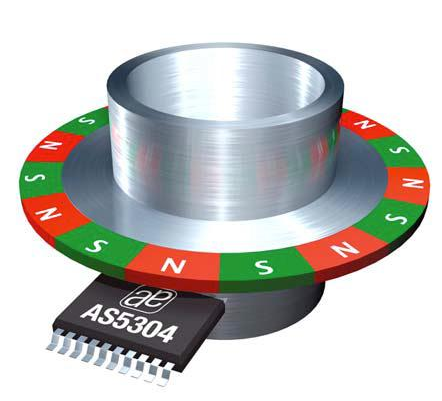
\includegraphics[width=0.5\textwidth]{data/magnetic_sensor.png}
\caption{Senzor AS5304 měřící natočení obruče na základě počítání pólů. Převzato
z~\cite{as5306}.}
\label{fig:magnetic-sensor}
\end{figure}

Výhodou tohoto způsobu měření je velice vysoká přesnost (řádově 10 bitů na
jednu otáčku). Bohužel, při pohledu na obrázek \ref{fig:magnetic-sensor} je
velice těžko představitelné jak umístit senzor na nápravu vagónu. Senzor by
musel být umístěn z~boku vozu, což by výrazně snižovalo jeho stabilitu.

Existují ale i~senzory, které se montují přímo na osu rotujícího předmětu viz
například senzor \textit{AS5306} \cite{as5306}. Takový senzor by pro účel této
práce byl nejvhodnější. Nepříznivým faktem ale je, že tyto senzory vyžadují
magnetický disk, přičemž ten nejmenší dosahuje průměru řádově $15$~mm
\cite{magnets}. Tento průměr je pro modelovou železnici bohužel příliš velký.

\subsection{Magnetický senzor \uv{cykloměřič}}
\label{subsec:wsm-senzor-cyclo}

Technologie tzv. \uv{cykloměřiče} byla historicky první metodou jak měřit
rychlost modelové lokomotivy. Tento senzor je založený na stejném principu jako
počítač rychlosti na cyklistickém kole. Na osu nápravy je upevněn magnet, ve
voze je pak hallova sonda. Magnet vyvolá při průchodu kolem hallovy sondy
zákmit v~magnetickém poli, který tato sonda detekuje. Na jednu otáčku nápravy
tak připadá jeden zákmit, cyklopočítač pak zaznamenává počty zákmitů.

Toto řešení je poměrně jednoduché na instalaci, množství mechanických prvků je
malé, na druhou stranu ale poskytuje poměrně malou přesnost -- zejména při
nižších rychlostech. Technologie \uv{cykloměřiče} se tedy pro potřeby této
práce také nejeví jako vhodná.

\subsection{Optický senzor}
\label{subsec:wsm-senzor-opto}

Třetí zvažovanou technologií je optický senzor. Tento senzor je proslulý svým
užitím v~optických myších. Pracuje na principu snímání obrazu podložky CCD
čipem a~porovnávání dvou obrazů pořízených v~krátkém časovém intervalu za
sebou. Ze dvou obrazů je pak určen rozdíl polohy myši.\footnote{Zajímavostí
je, že celá logika porovnávání dvou obrazů je v~takovýchto senzorech
implementována hardwarově.}

Toto řešení vypadá velice slibně, jeho obrovskou výhodou je absence jakýchkoliv
mechanických částí. Stačí namířit senzor na pražce a~jednoduše měřit jak se vůz
pohybuje. Pražce jsou navíc vůči štěrku mezi pražci velice dobře kontrastní,
porovnávání obrazů by tak mohlo být přesné (srovnejte s~pohybem optické
myši po takřka uniformním povrchu stolu nebo podložky pod myš).

Pro kalibrační vůz byl vybrán senzor \textit{ADNS-3050} \cite{adns-3050}.
Tento senzor byl mezi mnohými podobnými zvolen proto, že (1) má výstup sériovou
linkou a~(2) zvládá měřit vysoké rychlosti (vagón se typicky pohybuje o~něco
rychleji než myš).

Autor zakoupil senzory, osadil je na desku plošných spojů a~začal testovat
přesnost měření pomocí jednoduchého zapojení s~vývojovým kitem Arduino. Nemalou
výzvou bylo sehnat čočku, která autorovi umožní zaměřit pražce a~zároveň
ponechat senzor na ploše vagónu. Díky spolupráci s~Ústavem přístrojové techniky
AV ČR se však povedlo dostatečně malou čočku obstarat.

První měření ukázala, že pro dobrou funkci senzoru je třeba poměrně kontrastní
snímaná plocha a~poměrně intenzivní červené světlo (na to je CCD čip v~senzoru
nejcitlivější\footnote{Proto si optická myš přisvětluje červeným světlem.}).
Navíc se ukázalo, že hloubka ostrosti senzoru je nejvýše $1$~mm, což reálně
znemožňovalo měřit rychlost na kolejích, které nejsou zasypány štěrkem, ale
pouze připevněny k~podložce. Složitý optický senzor tak degradoval na zařízení,
jehož funkci by v~podstatě šlo obstarat pomocí jedné LED diody a~jednoho
fototranzistoru \footnote{Stačí jednoduše měřit intenzitu odraženého světla
a~zkoumat, jestli je senzor zrovna na pražci nebo mezi pražci.}.

Po několika měsících pokusů o~zprovoznění měření optickým senzorem autor naznal,
že s~tímto typem senzoru nebude schopen garantovat přesné a~spolehlivé měření.
Padlo tedy rozhodnutí tuto technologii opustit. Autor by rád zdůraznil, že
jednou z~hlavních motivací pro opuštění této technologie byla přílišná
komplexnost senzoru a~neschopnost ovlivňovat a~debugovat procesy uvnitř něj.

\subsection{Optozávora}
\label{subsec:wsm-senzor-optozavora}

\begin{figure}[h]

\includegraphics[width=0.3\textwidth]{data/clonka.pdf}
\caption{Příklad paprskového kola.}
\label{fig:wheel}
\end{figure}

Čtvrtá uvažovaná technologie senzorů je inspirována návrhem od kolegy modeláře
Petra Trávníka. Jejím základem je paprskové kolo (viz obr. \ref{fig:wheel})
upevněné na nápravě měřicího vozu. Paprskové kolo se otáčí spolu s~nápravou,
k~vozu je pak připevněna optozávora, která snímá průchod jednotlivých paprsků.
Klíčovým faktorem pro použitelnost této technologie jsou zejména technické
možnosti výroby dostatečného množství paprsků při zajištění rovnoměrnosti
rozestupu paprsků a~malé velikosti kola. Průměr kola by totiž neměl přesáhnout
$6$~mm (pro měřítko TT, 1:120).

Tato technologie sice obsahuje mechanické prvky, ale pořád je jich poměrně
málo. Při dostatečném počtu paprsků dosahuje dobré přesnosti, je jednoduchá,
a~tudíž jsou data z~ní snadno zpracovatelná. Optozávora je také levná a~relativně
snadno dostupná.

Ze všech zvažovaných technologií autor nakonec zvolil právě technologii
paprskového kola a~optozávory.

Nejvhodnější technologií pro výrobu takového kola je zřejmě leptání, protože
autor však nemá k~této technologii přístup, rozhodl se místo jednotlivých
paprsků kolo vyrobit dírkované. Jako vhodný kompromis bylo stanoveno
8 dírek na kolo, přičemž chyba v~umístění jedné dírky byla výrobou stanovena na
nejvýše $0,05$~mm. To jsou poměrně dobré výsledky.

Výkres kola je zobrazen v příloze \ref{fig:final-wheel}.

Drobným problémem pak bylo sehnat dostatečně malou optozávoru. Běžné optozávory
dostupné v~českých obchodech dosahují rozměrů cca $15\times6\times10$~mm
\footnote{Viz například
\url{https://www.gme.cz/optozavory-reflexni-optocleny}}. To je pro účely vozu
v~měřítku 1:120 zcela nepřijatelné. Po
průzkumu možných alternativ byl nakonec vybrán senzor
GP1S23 \cite{gp1s23:datasheet}, který byl dříve hojně montován do disketových
mechanik. Dnes je senzor běžně dostupný například na modulu k~vývojové desce
Arduino pod označením \textit{KY-010} \cite{ky-010}.

\section{Napájení}
\label{sec:wsm-napajeni}

Jedním z~klíčových faktorů, který určoval výslednou podobu měřicího vozu, bylo
napájení. Pro napájení elektroniky jsou 3 možnosti.

\begin{compactenum}
\item Napájení z~kolejí.
\item Napájení z~baterie.
\item Kombinace předchozích dvou (místo baterie lze případně použít kondenzátory).
\end{compactenum}

Výhody a~nevýhody jsou poměrně jasné: baterie má omezenou výdrž, napájení
z~kolejí je stálé. Na tomto místě je ale třeba zmínit, že napětí v~kolejích
sice je (téměř) trvale přítomné, ale zajistit jeho spolehlivé sbírání je
skutečně výzva. Sbírání je typicky realizováno plíšky s~kontakty na kola.
Na základě odhadnuté spotřeby měřicího vozu (viz níže) byla vytvořena modelová
zátěž a~indikace, jak dobře je sbírání schopno tuto zátěž \uv{uživit}.

Naměřená data bohužel byla naprosto tristní. Sbírání bylo realizováno skrze
hrotová ložiska, protože při použití sbíracích kontaktů přiložených přímo na
kolečko vzniká riziko, že tření mezi kontaktem a~kolem bude tak vysoké, že kolo
bude na kolejnici prokluzovat. A~to je v~kontextu faktu, že na tomto kole
probíhá měření rychlosti, naprosto nemyslitelné. Zátěž byla napájena cca $50 \%$
času a~to i~přes veškerou snahu o~přídavné kondenzátory a~případnou přídavnou
hmotnost pro zlepšení kontaktu vozu s~kolejemi.

Na základě těchto měření i~autorových předchozích zkušeností se sbíráním
u~přípojných vozů bylo rozhodnuto zkonstruovat vůz bez sbírání. Později byla
zvažována řešení zahrnující baterie i~sbírání dohromady, tato řešení se ale
ukázala jako příliš komplikovaná.

Poslední alternativou tedy zůstala baterie. Výzvou při použití baterie je
vměstnat co největší baterii do malého prostoru vozu. Minimální doba kalibrace
na jedno nabití byla stanovena na 3 hodiny. Jednou z~výhod baterie je to, že
vůz není nutné upravovat (instalovat sběrací kontakty) a~že vůz lze za jeho
plné funkčnosti bez problému sejmout z~kolejí a~například tak vyzkoušet
funkčnost senzoru.

Za technologii baterií byla zvolena LiPol.

Skutečnou výzvou se tak stalo vyrobit elektroniku tak, aby její spotřeba byla
vskutku malá (viz další kapitolu).

\section{Přenos dat do PC}
\label{sec:wsm-prenos-pc}

Dle požadavků na měřicí technologii (viz kapitolu \ref{chap:pozadavky}) je
nutné zajistit bezdrátový přenos dat ze senzoru. Primární technologií na straně
příjemce je pro účely této práce počítač, pokud se však podaří vybrat takovou
technologii, aby data mohla být přenášena například i~na mobilní telefon či
tablet, bude to pro měřicí vůz jen výhodou. Autor se proto rozhodl vyhnout se
proprietárním řešením pro bezdrátový přenos dat a~cílit na technologie, které
jsou běžně dostupné, ideálně přímo zabudované v~dnešních počítačích.
V~neposlední řadě je třeba zmínit, že nutnost pořizovat či stavět přijímač by
zvyšovala náročnost celého projektu, a to jak po stránce finanční, tak po
stránce výrobní.

S~tímto vědomím přicházejí v~úvahu 2 technologie:

\begin{compactenum}
\item Wi-Fi,
\item Bluetooth.
\end{compactenum}

\section{Platforma}
\label{sec:wsm-platforma}

Na základě požadavků vyplynuvších z~předchozích kapitol (senzor, přenos dat)
je nutné vybrat hardware, který bude umístěn do měřicího vozu.

\subsection{ESP-32}
\label{subsec:wsm-esp32}

Prvním kandidátem byl procesor \textit{ESP-32} \cite{esp-32}, jehož největší
výhodou je vestavěný Bluetooth a~WiFi. Jedná se o~poměrně výkonný procesor,
který lze taktovat až na $240$~MHz a~to dokonce na dvou jádrech!
\cite{esp-32:datasheet}

Autor pořídil \textit{ESP-32} vývojový kit a~začal zkoušet možnosti komunikace. Jako
primární komunikační kanál byl vybrán Bluetooth, jelikož vyžaduje oproti WiFi
menší režii spojenou s~ustanovením spojení. Tento problém by šel u~WiFi řešit
tím, že se měřicí vůz nepřipojuje k~již existující síti, ale sám síť vytváří.
Negativem tohoto přístupu je však ale to, že typicky není možné na počítači,
který přijímá signál z~měřícího vozu přes WiFi, být zároveň připojený do sítě
internet (přes WiFi). A~to je nanejvýš nepraktické.

Bluetooth na \textit{ESP-32} fungoval zdárně. Na ESP se podařilo aktivovat Bluetooth SPP
profil \cite{spp:specs}, takže se zařízení poměrně snadno spárovalo s~počítačem
a~tvářilo se jako sériová linka. Profil SPP byl vybrán, protože má
poměrně dobrou implementaci na celé škále operačních systémů a~vytváří dobrou
abstrakci pro použití z~jakéhokoliv programu. Téměř na každém operačním systému
je totiž možné \uv{otevřít sériovou linku}. Pokud by se podařilo zvolit pro
vývoj aplikace na počítač takový framework, který zvládá abstrahovat sériový
port nezávisle na cílové platformě, vzniklá aplikace by byla dokonale
multiplatformní.

Po nasazení profilu SPP se však ukázalo, že spotřeba \textit{ESP-32} je cca $80$~mA,
což jej dělá -- v~kontextu napájení z~baterie -- nepoužitelným. Bylo zvažováno
využít specifikace \textit{BLE (Bluetooth Low Energy)}, BLE však nemá
profil pro sériovou linku, takže by bylo nutné vytvořit profil vlastní. To
by znamenalo dodat specifikaci profilu do klientského zařízení (do počítače)
a místo abstrakce sériovou linkou přistupovat přímo k~zařízení Bluetooth.
Toto řešení bylo zamítnuto pro příliš velkou pracnost a~ztrátu elegance.

Autor ještě zvažoval, jak problém se spotřebou řešit pomocí sbírání či
zvětšení baterie, všechna navrhovaná řešení však byla příliš komplikovaná nebo
nefungovala dobře. ESP-32 tak bylo zavrhnuto.

\subsection{ATmega + HC-05}
\label{subsec:wsm-atmega}

Druhou volbou byla autorovi dobře známá rodina procesorů s~architekturou
\textit{AVR} názvu \textit{ATmega} \cite{avr}. Procesory rodiny \textit{ATmega}
jsou univerzální nízkopříkonové procesory, které jsou základem například
vývojové desky Arduino \cite{arduino}. Rodina procesorů \textit{ARmega} byla
zvolena také z~toho důvodu, že s~jejím programováním má autor předchozí
zkušenosti.

Procesory \textit{ATmega} ale bohužel neobsahují vestavěný modul pro
bezdrátovou komunikaci. Bylo tedy nutné využít externí Bluetooth modul
propojený s~procesorem pomocí sběrnice. Pro tento účel byl zvolen
běžně dostupný BT modul typu \textit{HC-05}. Výhodou tohoto modulu je jeho
dostupnost a~nízká cena, nevýhodou je to, že modul trpí neduhy typickými pro
celou řadu zařízení vyráběných v~Číně. K~modulu například není k~dispozici
kvalitní dokumentace a~v~Česku je to s~jeho dostupností horší. Každopádně
-- co se týče světové dostupnosti -- je na tom modul \textit{HC-05} velice
dobře. Autor zvažoval ještě další moduly (\textit{HC-06}, \textit{HC-07}), tyto
moduly by však pro účel této práce nepřinesly žádnou zásadní výhodu.

Autor experimentálně změřil, že spotřeba nespárovaného \textit{HC-05} modulu je
$42$~mA~$\pm$~$0,2$~mA, spotřeba spárovaného modulu je $20$~mA $\pm$ $2$~mA. To
jsou oproti ESP-32 výrazně příznivější čísla. Navíc se podařilo zajistit
spolehlivou funkci optozávory již při proudu $10$~mA, což je polovina proudu,
na který je senzor dimenzován \cite{gp1s23:datasheet}. S~přihlédnutím ke
spotřebě procesoru a~dalších drobných součástek by se měla pohybovat celková
spotřeba vozu kolem cca $30$~mA. Tato spotřeba byla uznána jako přijatelná.

Pro konstrukci měřicího vozu byla tedy vybrána platforma \textit{ATmega}
s~Bluetooth modulem \textit{HC-05}.

\section{Mechanika}
\label{sec:wsm-mech}

Vůz se bude po mechanické stránce skládat z~několika základních částí.

\begin{compactenum}
\item Perforované kolo připevněné na nápravě.
\item Optozávora připevněná k~vozu snímající perforované kolo.
\item Baterie.
\item Deska plošných spojů s~hlavní elektronikou.
\item Komunikační modul \textit{HC-05}.
\end{compactenum}

Jako vůz byl použit běžně dostupný vůz měřítka TT typu \textit{Nd}
\cite{vuz-nd}. Na jedné straně bylo extrahováno spřáhlo a~místo něj byla
k~nápravě umístěna optozávora. Optozávora je na vlastní miniaturní DPS, k~vozu
je DPS mechanicky připevněna lepidlem. Vůz \textit{Nd} je otevřený vůz, autor si
(minimálně v~prototypu) neklade za cíl měřicí elektroniku modelově maskovat. Na
plošině vozu je umístěna baterie, na ní je řídicí elektronika a~na ní je
komunikační modul. Celou situaci přehledně zobrazuje nákres
\ref{fig:vuz-nakres}

\begin{figure}[h]
TODO
\caption{Nákres mechaniky měřicího vozu.}
\label{fig:vuz-nakres}
\end{figure}

Rozměr plošiny vozu je $20\times80$~mm, což umožnilo instalaci LiPol baterie
o~kapacitě $500$~mAh (napětí $3,7$~V). Teoretická výdrž vozu je tedy cca $15$
hodin. Je však nutno poznamenat, že toto číslo je pouze teoretické, spotřeba
zařízení se výrazně liší ve spárovaném a~nespárovaném stavu, navíc níže
zjistíme, že baterii nevybíjíme až na její hranice. Předestřeme však již nyní
naměřenou hodnotu, tj. že spárovaný vůz vydržel reálně komunikovat $14$ hodin.
To je velice uspokojivý výsledek.

\section{Elektronika}
\label{sec:wsm-ele}

Základní požadavky na elektroniku měřicího vozu jsou:

\begin{compactenum}
\item Umět rychle a~přesně vyhodnocovat data z~optického senzoru.
\item Umět komunikovat s~modulem \textit{HC-05}.
\item Umožnit uživateli zařízení zapnout a~vypnout.
\item Umět měřit napětí na baterce.
\item Umět automaticky vypnout zařízení v~případě vybití baterie.
\item Zobrazovat stav vozu LE diodami.
\item Umožnit nabíjet baterii.
\end{compactenum}

Tyto požadavky na elektroniku jsou víceméně intuitivní, jen u~posledního
doplňme, že jeho motivací je to, aby uživatel nemusel odpojovat baterii od
elektroniky a~nabíjet jí externě. Tím se výrazně sníží riziko omylného
přepólování, nesprávného zacházení s~baterií ze strany uživatele a~mechanického
poškození vozu vlivem časté manipulace s~kabely a~konektory.

Schéma desky plošných spojů je k~nahlédnutí v~příloze \ref{fig:wsm-sch}. Nyní
budou krátce popsány jednotlivé prvky schématu a~jak tyto prvky přispívají
k~naplnění požadavků.

Hlavní součástkou na DPS je procesor \textit{ATmega328p}
\cite{atmega328p:datasheet}.  Tento konkrétní typ byl vybrán, protože je
poměrně moderní a~je dnes montován do vývojových desek Arduino, tudíž je jeho
cena díky vysokému počtu produkovaných kusů malá. Procesor se stará o~všechnu
logiku na desce.  Signál z~optozávory je připojen na pin \textit{ICP}, který je
speciálně určen k~tomu, aby přesně a~rychle měřil periodu vstupního signálu.
Procesor dále měří napětí na baterce, které je ale nejprve nutné srazit
napěťovým děličem. Při vývoji hardwaru byla v~jednu chvíli překážkou přesnost
napěťové reference, nakonec ale byla zvolena jako napěťová reference přímo
napájecí napětí procesoru, které by mělo kolísat nejvýše $\pm 2$ \%
\cite{ldo:datasheet}.

Součástí schématu je dále nabíjecí obvod \textit{MCP73831}, který byl vybrán
zejména pro jeho velice malé rozměry.

Za nabíjecím obvodem je ochrana proti přepólování (tranzistor \textit{T1A})
a~dále zapínací a~vypínací obvod celé elektroniky. Tento obvod je inspirován
projektem \textit{RB3201} \cite{rb3201} od kolegů z~Robotiky Brno
\cite{roboticsbrno}.

Napětí pro procesor je vytvářeno obvodem LDO\footnote{Low-dropout regulator}
(obvod \textit{IC3}), procesor pracuje na napětí $3,3$~V. Tato konstrukce
s~sebou nese zásadní omezení pro čerpání baterie: napětí na baterii nikdy nesmí
klesnout pod $3,5$ V. Tato hodnota zahrnuje i~korekce vypočítané z~nepřesnosti
výstupu LDO, jedná se tedy o~\textit{napětí, které měří procesor}. Jakmile
procesor na baterce změří méně než $3,5$~V, musí se odpojit. Jinak hrozí
pokles referenčního napětí na AD převodníku, který měří napětí na baterii.

DPS dále obsahuje konektory pro periferie, testovací konektory, testovací
plošky a~LE diody.

Kompletní materiály k~elektronice jsou k~dispozici pod licencí \textit{CC BY-SA
4.0} na serveru GitHub \cite{wsm-pcb}.

\section{Princip měření}
\label{sec:wsm-mer-princip}

První pohled na měření rychlosti vozidla by mohl vycházet z~analogie
s~tachometrem na kole: stačí měřit kolik pulzů za sekundu se na senzoru vytvoří
a podle toho počítat rychlost. Ukazuje se však, že tato metoda měření nedosahuje
zejména při malých rychlostech dostatečné přesnosti.

Mnohem přesnějším způsobem měření je měřit periodu mezi jednotlivými pulzy ze
senzoru. Zde vyvstává otázka, jestli bude procesor schopný měřit i~rychlosti
okolo modelových rychlostí cca $120$~km/h.

Uvažme tedy modelovou rychlost vozidla $v_m = 120$~km/h $\doteq$ $33,3$~m/s.
Protože se jedná o~rychlost v~modelu, pro získání reálné rychlosti $v$ je třeba
uvážit modelové měřítko $c$ (např. $c = 1:120$, $c = 1:87$).

$$v = v_m \cdot c$$

Aplikováním základních vztahů platících pro rovnoměrný pohyb po kružnici snadno
dostáváme vztah

$$v = \omega r = 2 \pi f r.$$

Oba předchozí vztahy už stačí jen dát do rovnosti, vyjádřit výslednou frekvenci
a tuto frekvenci vynásobit počtem děr na kole. Získáme tak nejvyšší frekvenci,
kterou by měl vůz být schopen s~přehledem měřit.

Po dosazení nejhorších hodnot (měřítko $1:87$, průměr kola $8$~mm, rychlost
$120$~km/h) dostáváme frekvenci přibližně $220$~Hz. To je ve srovnání
s~kmitočtem krystalu procesoru $f_{CLK} = 3,6864$~MHz zanedbatelná frekvence,
kterou bude možné s~přehledem měřit velice přesně.

Naměřená hodnota bude zaznamenávána do paměti procesoru a~jednou za pevně daný
interval bude odeslána do počítače. Tento interval byl zvolen na $100$~ms.

Z~naměřené periody $T$ lze modelovou rychlost spočítat dle vztahu
\ref{prepocet}

\begin{equation}
v_m = 3.6 \cdot \frac{\pi d F_{CPU}}{T h c p},
\label{prepocet}
\end{equation}

kde $d$ je průměr modelového kola, $F_{CPU} = 3686400$~MHz je frekvence
krystalu k~procesoru, $h = 8$ je počet děr v~kole, $p = 64$ je
\textit{prescaler} časovače a~$c$ je modelové měřítko (viz výše).

Spolu s~aktuální rychlostí je vhodné měřit také ujetou vzdálenost. A~protože
výpočet vzdálenosti z~rychlosti až v~počítači by mohl být vzhledem k~vzorkování
rychlosti po $100$ms intervalech nepřesný, je vhodné výpočet ujeté dráhy
implementovat přímo do měřicího vozu. Druhou měřenou hodnotou je tedy čítač
pulzů senzoru. Hodnota čítače je 32-bitové číslo, které je do počítače zasíláno
jednou za $500$~ms. Příslušné přepočty na hodnoty v~uživateli čitelných
jednotkách jsou pak jak v~případě rychlosti tak v~případě ujeté vzdálenosti
ponechány až na počítači, neb ten má spoustu výpočetních prostředků
a~nepotřebuje realizovat časově citlivé operace. Navíc odpadá problém
s~přenášením hodnot parametrů (průměr kola, měřítko) do měřicího vozu
a~komunikace tak může být pouze jednosměrná. Reálnou dráhu $s$ lze pak z~počtu
kmitů vypočítat pomocí vztahu \ref{real-dist}

\begin{equation}
s = \frac{i \pi d}{h}
\label{real-dist}
\end{equation}

kde $i$ je počet kmitů, $d$ je průměr modelového kola a~$h = 8$ je počet děr
v~kole.

Pro komunikaci s~počítačem byl navrhnut vlastní binární protokol inspirovaný
protokolem XpressNET \cite{xpressnet-specs}. Jedná se o~jednoduchý protokol, který
v~prvním bytu zprávy určí délku zprávy, poslední byte zprávy je pak její
kontrolní součet (\textit{XOR}). Protokol umí ve verzi 1.0 zasílat informace o:

\begin{compactenum}
\item aktuální rychlosti,
\item ujeté vzdálenosti a
\item napětí na baterce.
\end{compactenum}

Zajímavým aspektem protokolu je fakt, že používá kódování \textit{7B8B}
a~nejvýznamnější bit nechává vždy nastavený na $1$. Důvodem pro tuto vskutku podivnou
vlastnost je fakt, že modul \textit{HC-05} interpretuje hodnoty bytů jako
ASCII znaky a~některé znaky odmítne přenést (např. \texttt{0x04} \textit{End
of transmission}). Proto byla použita pouze polovina rozsahu jednoho
bytu, která neobsahuje kontrolní znaky, konkrétně interval $128$--$255$.

Kompletní specifikace protokolu je k~dispozici online
\footnote{\url{https://github.com/kmzbrnoI/wsm-fw/blob/master/protocol.md}}.

\section{Firmware}
\label{sec:wsm-fw}

Na poli Embedded System mezi programovacími jazyky dominují zejména jazyky C
a~C++ a~to především díky přímočarému provázání příkazů jazyka přímo
s~výpočetními prostředky a~periferiemi mikrokontroléru. Z~relativní
jednoduchosti úkonů, které bude procesor řešit, plyne také poměrně malá
velikost jeho programu. Spolu s~faktem, že s~programováním procesorů rodiny
AVR v~programovacím jazyce C má autor práce zkušenosti, tento argument rozhodl
pro programovací jazyk C.

Firmware procesoru je -- podobně jako elektronika -- koncipován jako
opensource. Je dostupný pod licencí \textit{Apache License v2.0} \cite{wsm-fw}.

Pro kompilaci je využit standardní kompilátor \texttt{avr-gcc}, pro nahrávání
firmwaru do procesoru je využit program \texttt{avrdude}. Deska
plošných spojů je vybavena programovacím konektorem, procesor je tedy možné
programovat až v~desce. To umožňuje snazší výrobu desek a~především výrazně
usnadňuje vývoj vozu (firmware je možno kdykoliv aktualizovat).

Základní činnost procesoru lze shrnout do několika bodů.

\begin{enumerate}
\item Procesor pomocí přerušení a~využití speciálního pinu \textit{ICP}
měří periodu mezi jednotlivými pulzy senzoru.

\textit{ICP} je speciální mód časovače 1. V~tomto režimu časovač čítá a~při
vzestupné hraně na pinu \textit{ICP} velice rychle (hardwarově, bez generace
přerušení) zkopíruje hodnotu čítače časovače do registru procesoru. Poté je
vyvoláno přerušení, ve kterém je obsloužena naměřená hodnota. Konkrétně je od
této hodnoty odečten čas předchozího pulzu a~tím pádem je určena perioda
vstupního signálu. Perioda je uložena k~budoucímu odeslání do počítače.

\textit{Více o~dalším zpracování dat lze nalézt v~sekci
\ref{subsec:wsm-kompenzace}.}

\item V~primární \texttt{while} smyčce programu se nacházejí časově nekritické
operace (primární smyčka totiž může být kdykoliv přerušena). Ve
smyčce se každých $100$~ms odesílá aktuální rychlost do počítače, dále se každých
$500$~ms odesílá informace o~ujeté vzdálenosti a~každých $5$~s se měří napětí
na baterce.

\end{enumerate}

\section{Prototyp vozu}
\label{sec:wsm-prototype}

Na základě výše uvedených požadavků a~specifikací se podařilo vytvořit prototyp
měřicího vozu. Tento prototyp je vyobrazen na obrázku \ref{fig:vuz-photo}.

Tabulka \ref{tab:wsm-params} shrnuje klíčové parametry měřicího vozu.

\afterpage{

\begin{figure}[t!]
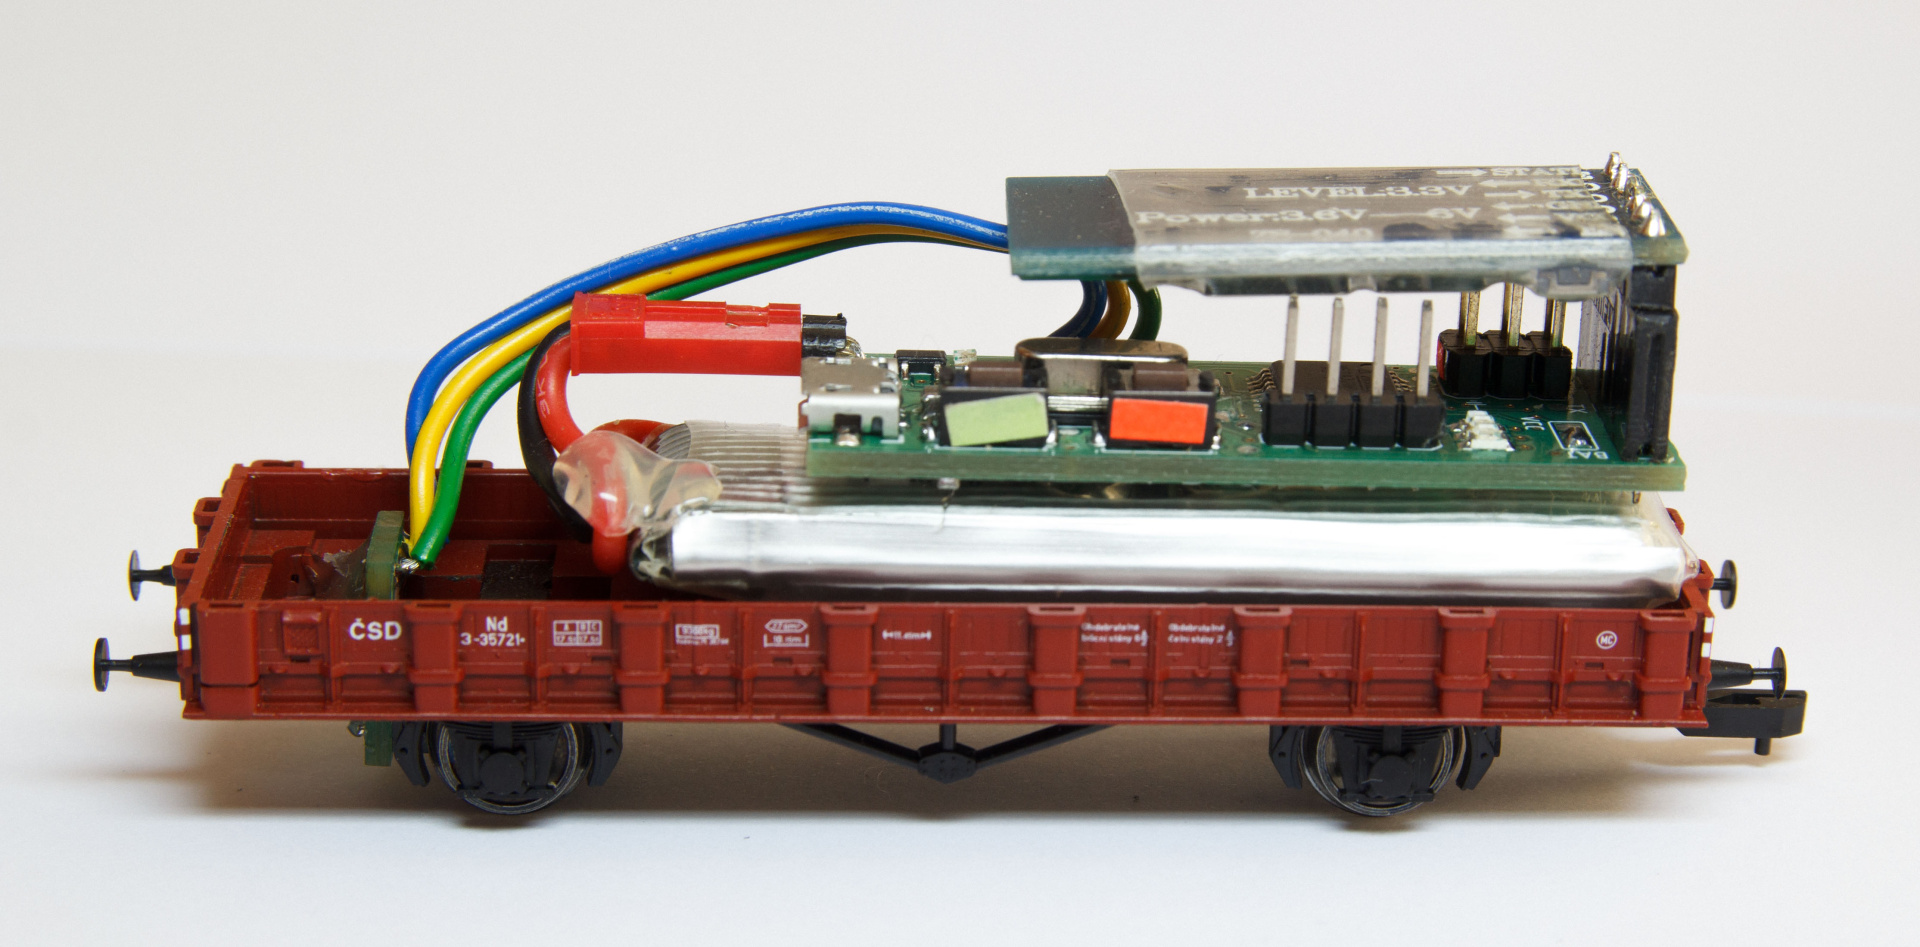
\includegraphics[width=\textwidth]{data/wsm_3d.jpg}
\caption{Fotografie prototypu měřicího vozu.}
\label{fig:vuz-photo}
\end{figure}

\begin{table}[h!]
	\begin{tabularx}{\textwidth}{lrl}
		\toprule
		Parametr & Hodnota & Jednotka \\
		\midrule
		Rozměry vozu\footnote & 98 $\times$ 25 & mm \\
		Spotřeba vozu při nespárovaném BT & 55 & mA \\
		Spotřeba vozu při spárovaném BT & 33 & mA \\
		Kapacita baterie & 500 & mAh \\
		Výdrž baterie & 14 & h \\
		Pracovní napětí baterie & 3,5--4,2 & V \\
		Využitá kapacita baterie & > 90 & \% \\
		Minimální měřitelná rychlost & 4 & modelový km/h\\
		Maximální měřitelná rychlost\footnote & 300 & modelový km/h\\
		Odhadovaná cena elektroniky & 500 & Kč\\
		\bottomrule
	\end{tabularx}
	\caption{Přehled základních parametrů měřicího vozu.}
	\label{tab:wsm-params}
\footnotetext[1]{Rozměr přes nárazníky.}
\footnotetext[2]{Účelové omezení ve firmwaru,
senzor zvládá měřit alespoň do 1000 modelových km/h.}
\end{table}
\newpage
} % end of argument of `\afterpage` command

Finální podobu vozu ovlivňovaly nejvíce ze všeho požadavky na malé rozměry všech
komponent měřicího vozu, dalším důležitým faktorem pak bylo napájení -- tedy
sehnat takovou baterii, která se do vozu vhodně vejde a~poskytne kapacitu
alespoň na několik hodin kalibrace.

Po vyrobení vozu byla provedena \uv{kalibrace} samotného vozu -- tedy určení
konstant uvedených ve vztahu \ref{prepocet}. Pro dosažení maximální přesnosti
se totiž nelze spoléhat zejména na měření průměru kola pouhým posuvným
měřidlem, rozdíly v~průměru kola v~řádu setin milimetru totiž způsobují rozdíly
v~modelové rychlosti v~řádu desetin modelových km/h. Autor tedy přistoupil ke
změření počtu pulzů na rovné koleji o~délce 1 m\footnote{Délka byla měřena
konvenčním svinovacím metrem.}. Postupně byly naměřeny hodnoty $317$, $317$,
$316$, $316$ a~$316$. První tři hodnoty byly měřeny na jednom úseku trati
v~různých směrech pohybu, zbylé 2 hodnoty byly pro eliminaci chyby měřeny na
jiném úseku trati, opět každá hodnota v~jiném směru pohybu vozu v~úseku a~na
rovné koleji bez jakýchkoliv nerovností.

Po zprůměrování pěti měření byl tedy průměr kola dle vztahu \ref{real-dist}
stanoven na $8,05$~mm, kterážto konstanta je použita v~budoucích programech.

\section{Naměřená data}
\label{sec:wsm-data}

Měření rychlosti se ukázalo býti funkčním, vůz pravidelně posílal naměřená
data, rychlost se pohybovala v~odhadovaných intervalech. V~naměřených datech
byla ale vidět poměrně silná oscilace rychlosti, jejíž perioda byla řádově
vyšší desetiny sekundy. Tato oscilace vykazovala amplitudu až
modelových 5~km/h, což je pro účely kalibrace zcela nevyhovující.

Autor tedy přistoupil ke zkoumání příčin této oscilace a~snaze o~jejich
odstranění. Autor upravil firmware v~procesoru tak, aby zasílal do počítače
každou naměřenou hodnotu a~v~počítači tak bylo možné vyhodnocovat surová data.

Při bližším pohledu na pohybující se vůz si šlo všimnout, že vůz ve spřáhlu
s~lokomotivou poměrně intenzivně pruží. To je dáno jak mechanickou konstrukcí
spřáhla, tak tím, že vůz i~lokomotiva obsahují kinematiku\footnote{Kinematika
je mechanismus uchycení spřáhla v~lokomotivě, ve kterém je spřáhlo k~rámu
lokomotivy připevněno přes pružiny, které zaručují natočení spřáhla při
průjezdu obloukem.}.
Autor tedy přistoupil k~nahrazení spřáhla pružného za spřáhlo pevné. Tento krok
pomohl ke snížení amplitudy oscilace, avšak oscilace rychlosti byla nadále
přítomná.

Ukázalo se tedy, že pro efektivní proces kalibrace bude nutné na kalibrované
lokomotivě vždy vyměnit spřáhlo. Toto zjištění je nepříjemné, neboť
jakákoliv nadbytečná manipulace s~kalibrovaným modelem zvyšuje šanci jeho
poškození, pragmaticky vzato však autor usuzuje, že se jedná o~přijatelné
riziko. Dnešní lokomotivy jsou na výměnu spřáhla dobře uzpůsobené, spřáhla
typicky bývají v~šachtách a~tak výměna spřáhla nepřináší až tak velká rizika.

Další zvažovanou možností bylo vůz tlačit přímo \uv{nárazník na nárazník},
ukázalo se však, že pro pevné spojení s~lokomotivou by bylo třeba vůz zatížit
řádově o~vyšší desítky gramů, což je zejména při omezených prostorech ve vozu
nereálné. Další možností je přidat soupravu se zátěží ještě před vůz a~tlačit
tak celý vlak, tuto možnost však autor vyhodnotil jako nepraktickou (bylo by
třeba mít k~dispozici další vozy, kalibrační vůz se tedy stává nekompaktní).

Naměřená data však stále vykazovala oscilaci v~řádu 5 \%, konkrétně perioda
vykazovala chybu například $2000 \pm 100$ (pro modelových 20~km/h) ticků
časovače 1. Chyba se navíc měnila s~naměřenou rychlostí a~to tak, že při
vyšších intervalech (menší rychlost) byla chyba větší než při kratších
intervalech (větší rychlost).

\begin{figure}[h]
\input{graph/speed_analog.tex}
\caption{Průběh naměřené periody a~modelové rychlosti v~čase v~analogovém
režimu.}
\label{fig:speed-analog}
\end{figure}

Graf \ref{fig:speed-analog} zachycuje průběh periody a~modelové rychlosti
v~čase. Každý celek bodů na zhruba stejné souřadnici $y$ zachycuje rychlost
vozidla při jednom napětí na jeho motoru. Rychlost je měřena na vozidlu
s~motorem připojeným přímo ke koleji (tzv. varianta \textit{analog}, bez
dekodéru), aby se eliminoval případný vliv dekodéru. Čas na ose $x$ je čas
příjmu signálu do počítače. Vůči reálnému času zachycení signálu procesorem se
tento čas může mírně lišit, avšak rozdíl by měl být skutečně nepatrný.

Krom pravidelné oscilace rychlosti je na grafu místy patrný globální
\uv{obloukový} trend. Tento jev lze vysvětlit tím, že v~průběhu měření
rychlosti vozidlo zrovna najíždělo do oblouku, takže se jeho rychlost díky
odstředivé síle zmenšila. Komentovaný jev je pro proces kalibrace parazitický,
autor se jeho vlivu obával už při prvních teoretických návrzích vozu. Později
se však ukázalo, že při kalibrování na oválu o~dostatečně velkých poloměrech
oblouků je změna rychlosti vlivem průjezdu obloukem minimální, resp. BEMF ji
okamžitě vykompenzuje. Pokud by uživatel přeci jenom chtěl kalibrovat na
obloucích o~malých poloměrech, nabízí se možnost výběru používaných
a~nepoužívaných měřicích úseků na kalibračním okruhu. Stručně řečeno se bude
měřit rychlost jen ve vybraných úsecích (typicky rovných úsecích), údaj
o~poloze vozidla bude založen na vyčítání ujeté vzdálenosti vozidla, viz sekci
\ref{sec:wsm-mer-princip}.

Všimněte si v~grafu \ref{fig:speed-analog} také průběhu naměřené rychlosti.
Díky způsobu, jakým je naměřená perioda přepočítávána na modelovou rychlost
(\ref{prepocet}) dochází k~dobré eliminaci velkých chyb při malých rychlostech,
avšak chyby v~periodě u~větších rychlostí -- přestože jsou v~absolutních
hodnotách o~mnoho menší -- způsobují mnohem větší oscilace modelové rychlosti.

Pro oscilaci rychlosti bylo vytvořeno několik hypotéz.

\begin{enumerate}
\item Oscilace je způsobena nepřesností měření.

Oscilace naměřených intervalů je v~řádu stovek ticků časovače procesoru, je tedy
zřejmé, že se nemůže jednat o~chybu měření v~procesoru. Dalším zdrojem chyb
může být mechanická nepřesnost v~poloze děr v~perforovaném kole, či chyba
v~umístění kola (natočené kolo).

Pokud je tato hypotéza pravdivá, chyba v~datech by se u~měřicího vozu měla
projevit, ať už je zdrojem pohybu vozu cokoliv. Autor tedy přistoupil k~tomu,
že do vozu prostě \uv{šťouchnul} a~sledoval jeho rychlost během zpomalování.
Tuto rychlost zobrazuje graf \ref{fig:speed-zduch}.

\begin{figure}[h]
\input{graph/speed_zduch.tex}
\caption{Průběh naměřené periody zpomaleného pohybu.}
\label{fig:speed-zduch}
\end{figure}

Všimněte si, že rozsah na ose $y$ je asi $4 \times$ menší než rozsah v~grafu
\ref{fig:speed-analog}, přesto není oscilace na tomto grafu patrná.

Osilace tedy není způsobena chybou v~konstrukci měřicího vozu.

\item Oscilace je způsobena BEMF regulátorem v~dekodéru.

Jak bylo zmíněno v~kapitole \ref{sec:det-static}, každý dekodér v~sobě má PID
regulátor, který zajišťuje udržování rychlosti hnacího vozidla při rozdílném
počtu zavěšených vozů, resp. při rozdílné zátěži. Jako každý PID regulátor,
i tento regulátor nemusí být dobře nastaven, výrobce dekodéru ostatně často
vůbec netuší, do jakého modelu bude jeho dekodér osazen.

Tuto hypotézu však vyvrací fakt, že oscilace se projevuje i když měříme rychlost
vozidla bez dekodéru -- v~tzv. režimu analog, kdy připojujeme napětí v~kolejích
přímo na motor.

\item Oscilace je způsobena charakteristikou motoru a~mechanickými vlastnostmi
modelu.

\begin{figure}[h]
\input{graph/speed_detail.tex}
\caption{Detailnější pohled na oscilace rychlosti.}
\label{fig:speed-presny}
\end{figure}

Zde se pouštíme už na poměrně tenký led. Z~grafu \ref{fig:speed-presny} je
patrné, že měření frekvence oscilace je za hranou možností měřicího
vozu. Počet děr v~perforovaném kolu je na přesné měření frekvence totiž příliš
malý.

Poslední hypotézou tedy zůstává to, že oscilace, která je patrná v~grafu,
je přímým důsledkem postupné aktivace pólů motoru, střídy signálu do motoru,
případně důsledkem nedokonalých převodů lokomotivy a~šíření vibrací přes
koleje až do vozu.

Fakt, že amplituda oscilace je při nižších rychlostech vyšší lze vysvětlit tím,
že vozidlo má při nižších rychlostech menší setrvačnost a~tudíž se pulzní
charakter regulace a~nepřesnosti v~převodech více projevuje.

Jako drobnou poznámku autor uvádí, že z~naměřených dat nejspíš (!) plyne,
že perioda oscilace se liší u~různých vozidel. Měření na různých vozidlech
proběhlo, autor ale znovu podotýká, že měření frekvence oscilace je za hranou
možností měřicího vozu.

\end{enumerate}

\subsection{Kompenzace chyb}
\label{subsec:wsm-kompenzace}

\begin{figure}[h]
\input{graph/speed_prumer.tex}
\caption{Naměřená data za použití průměrovací metody.}
\label{fig:prumer}
\end{figure}

Z~naměřených dat vyplývá, že v~signálu se vyskytuje určitá periodická chyba,
kterou by bylo vhodné kompenzovat. Za tímto účelem vznikl návrh průměrovací
metody \textit{kluzné okno}. Tato metoda je implementována v~produkční verzi
kalibračního vozu, princip její činnosti je následující:

\begin{compactenum}
\item Měř počty ticků a~jejich periodu ve $100$ms oknech.
\item Každých $100$~ms přepni na nové okno.
\item Data do počítače průměruj z~posledních $10$ oken, tedy celkem z~$1$~s.
\end{compactenum}

Tato metoda je poměrně známá, zajímavou věcí na implementaci v~měřicím vozu
jsou výše uvedené konstanty. Sto milisekund proto, aby data v~počítači byla
vidět v~rozumně \textit{reálném čase} a~naopak příliš nezahlcovala komunikační
kanál, Jedna sekunda proto, že se jedná o~latenci, kterou je uživatel ještě
schopen tolerovat, navíc za tento čas obvykle nastane alespoň jedna perioda
signálu (viz naměřená data v~grafech výše).

O~přesné přepínání oken se v~procesoru stará časovač 0.

Průběh naměřené periody a~vypočítané rychlosti za použití průměrovací metody
zachycuje graf \ref{fig:prumer}. Srovnejte s~grafem \ref{fig:speed-analog}.


\chapter{Software} \label{chap:sw}
Pro potřeby této práce byly vytvořeny 2 aplikace. První aplikace je
demonstrační aplikací k~měřicímu vozu, tato aplikace pouze zobrazuje naměřená
data. Druhá aplikace je o~mnoho komplexnější a řeší přímo problém automatické
kalibrace.

\section{Volba nástrojů}
\label{sec:sw-nastroje}

Zásadní otázkou, kterou je třeba zodpovědět před programováním aplikace, je
jaký programovací jazyk a případně framework zvolit. Zde měl autor poměrně
jasný požadavek na programovací jazyk: jazyk musí mít poměrně silný typový
systém tak, aby spousta kontrol proběhla již během překladu. Důvodem pro tento
argument je fakt, že autor vyrábí aplikaci, které je tzv. \textit{kritická}.
V kontextu této práce to znamená, že vlivem chyby v aplikaci může dojít
k nemalým materiálním škodám na kalibrovaném modelu (ceny vybraných
malosériových modelů se pohybují až v~desítkách tisíc Kč).

Dalším přirozeným požadavkem bylo, aby programovací jazyk měl rozumnou podporu
pro komunikaci se sériovým portem, neboť toto rozhraní bude použito pro
komunikaci s měřicím vozem a digitální centrálou DCC.

Dalším kritériem při výběru programovacího jazyka byla jeho předchozí znalost
autorem práce. Zejména u kritických aplikací je totiž nanejvýš důležité, aby
programátor vědět, co dělá, když píše kód.

Při rozmýšlení nad technologií aplikace bylo rozhodnuto, že program by měl
mít grafické uživatelské rozhraní, neboť je nanejvýš vhodné zobrazovat přehledně
aktuální průběh kalibrace a neboť jsou běžní uživatelé na GUI aplikace zvyklí.

Zásadní je pak otázka typu aplikace. Autor uvažovat aplikace desktopové,
mobilní, webové, dokonce i embedded! U embedded aplikací je nevýhoda, že
obsluha s aplikací typicky nemůže příliš interagovat, u mobilních aplikací
je v kontextu této práce omezující zejména zobrazovací plocha zařízení, na
kterou se jednoduše nevejde tolik dat, kolik by aplikace chtěla zobrazovat.
Navíc vývoj pro jiné zařízení, než na kterém kód píšete, vždy přináší nějakou
režii navíc.

Výhodou webové aplikace by byla snadná přenositelnost na jiné počítače,
aplikace by dokonce mohla být přístupná i z mobilního zařízení. Bohužel, proti
tomuto formátu aplikace hovoří fakt, že autor práce nemá s webovými aplikacemi
dostatečné zkušenosti a už vůbec si netroufá v nich psát kritický kód.
Oproti desktopovým aplikacím jsou interaktivní webové aplikace navíc o něco
složitější (zejména co se týče předávání signálů z GUI).

Další možností pak byly desktopové aplikace. Vzhledem k požadavkům uvedeným
výše a k faktu, že se jedná už o trochu rozsáhlejší projekt, jako nejvhodnější
se autorovi jevil jazyk \texttt{C++} s použitím frameworku \texttt{Qt}.
Argumentem pro tento framework byly dobré osobní reference, které na
\texttt{Qt} autor práce dostal os kolegů. Ukázalo se také, že Qt poskytují
nejde výbornou multiplatformní podporu pro GUI, ale také stejnou
multiplatformní podporu pro sériový port. Bylo tedy rozhodnuto, že výsledná
aplikace bude psána v programovacím jazyce \texttt{C++} (konkrétně
\texttt{C++14}) za použití frameworku \texttt{Qt} a bude multiplatformní
(minimálně mezi OS \texttt{Window} a \texttt{Linux}). Důvodem pro
multiplatformnost je především autorova záliba v Linuxu a touha udělat aplikaci
dostupnou i pro běžné smrtelníky.

\section{WSM Speed Reader}
\label{sec:sw-wsm-speed-reader}

První aplikací je \textit{WSM Speed Reader} -- jednoduchý zobrazovač vyčtených
dat. Aplikace se skládá z~jednoho okna a je především typu
\textit{proof-of-concept}. GUI aplikace je zachyceno na obrázku
\ref{wsm-speed-reader-gui}.

TODO figure: wsm-speed-reader-gui

Aplikace se připojuje k sériovému portu, ze zadaných parametrů vypočítává
rychlost a ujetou vzdálenost vozidla a tyto údaje zobrazuje. Umožňuje ukládání
vyčtených dat do souboru (především pro vývoj) a ukládání nastavení aplikace
do konfiguračního souboru. Aplikace je volně dostupná pod licencí Apache
License v2.0\ref{wsm-speed-reader}.

\section{Automatic Calibration}
\label{sec:sw-wsm-auto-calib}


\printbibliography[heading=bibintoc]

\appendix
\chapter{Appendix} \label{chap:appendix}
\vspace{-2em}

\begin{figure}[H]
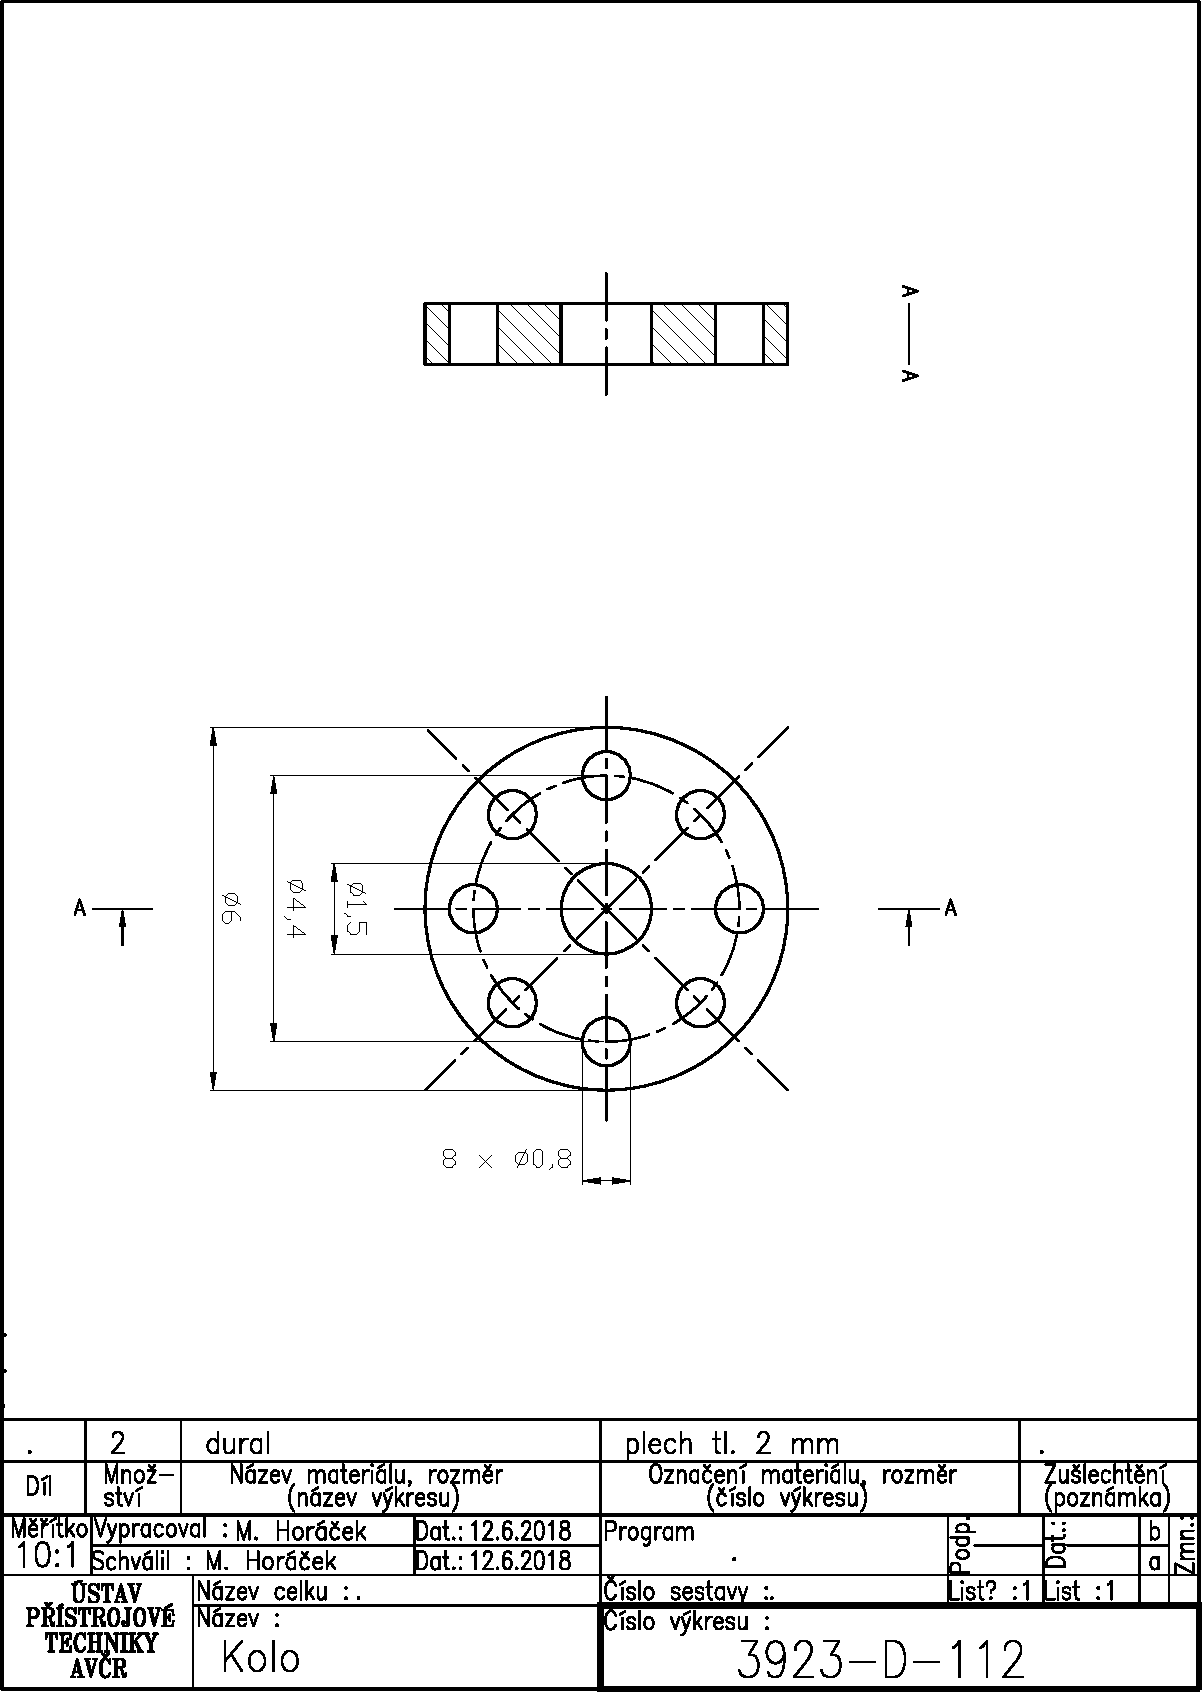
\includegraphics[width=0.95\textwidth]{data/wheel.pdf}
\caption{Výkres perforovaného kola. Autor: Miroslav Horáček.}
\label{fig:final-wheel}
\end{figure}

\begin{figure}[h]
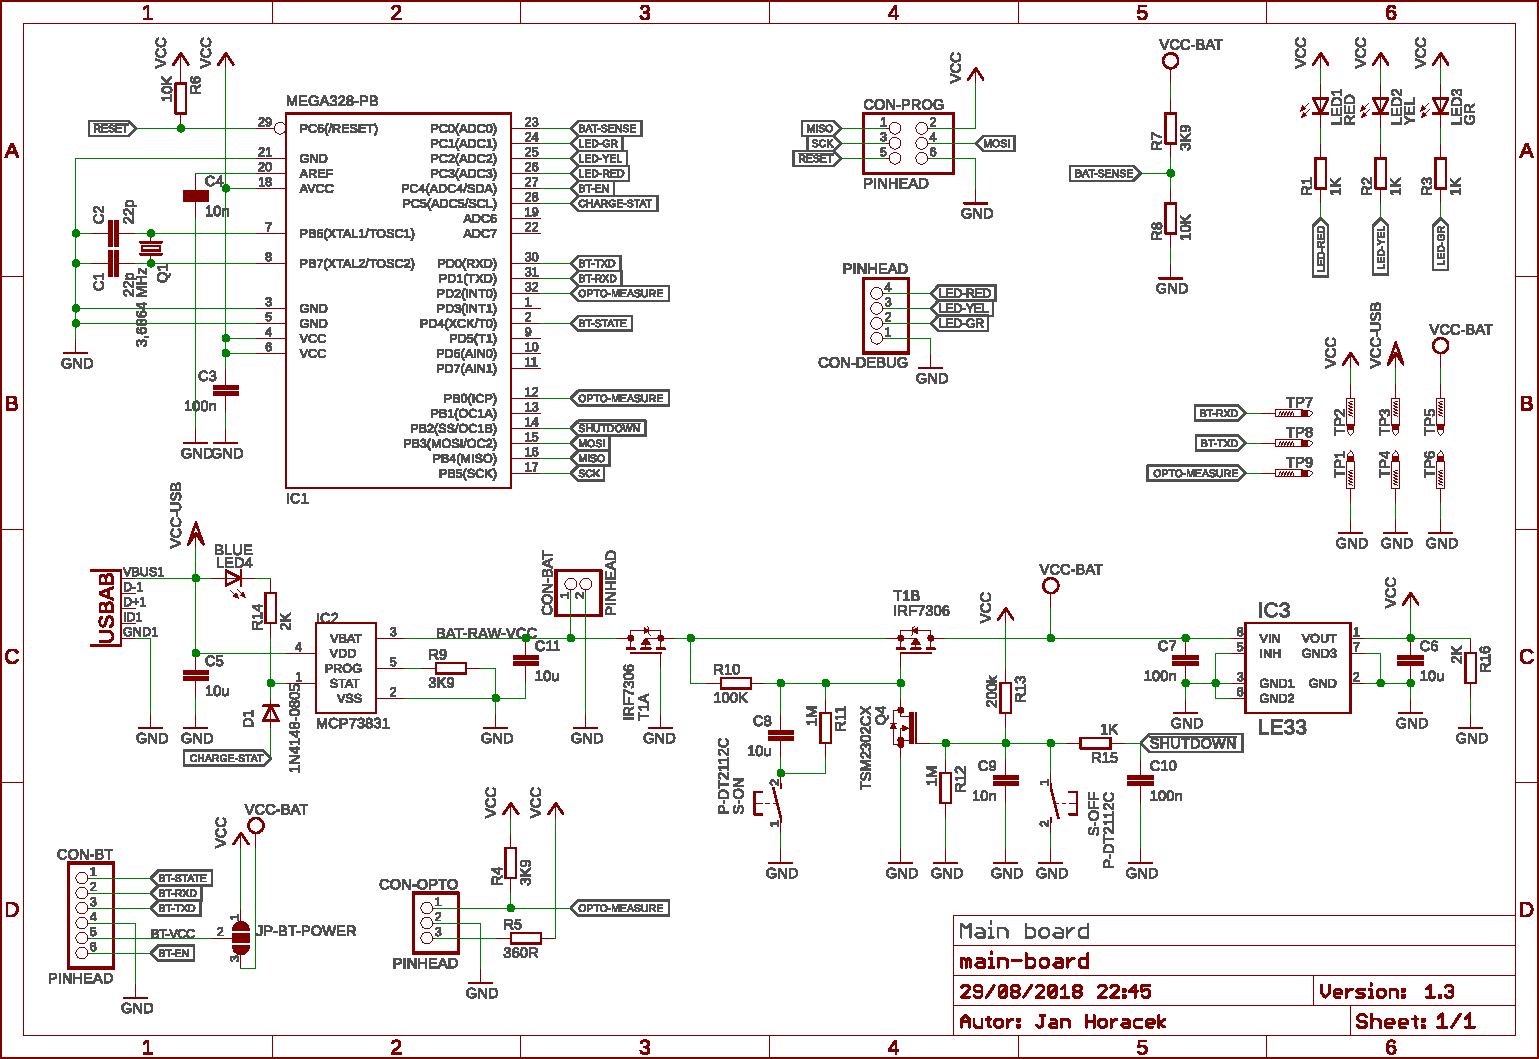
\includegraphics[angle=90,width=\textwidth]{data/wsm_main_board_v1_3.pdf}
\caption{Schéma hlavní DPS měřicího vozu.}
\label{fig:wsm-sch}
\end{figure}

\begin{table}[h]
	\begin{tabularx}{0.66\textwidth}{rrX}
		\toprule
		Jízdní stupeň & Rychlost [modelový km/h] \\
		\midrule
		1 & 1 \\
		2 & 2 \\
		3 & 4 \\
		4 & 6 \\
		5 & 8 \\
		\textbf{6} & \textbf{10} \\
		7 & 12 \\
		8 & 15 \\
		9 & 17 \\
		\textbf{10} & \textbf{20} \\
		11 & 22 \\
		12 & 25 \\
		\textbf{13} & \textbf{30} \\
		14 & 35 \\
		\textbf{15} & \textbf{40} \\
		16 & 45 \\
		\textbf{17} & \textbf{50} \\
		18 & 55 \\
		\textbf{19} & \textbf{60} \\
		20 & 65 \\
		\textbf{21} & \textbf{70} \\
		22 & 75 \\
		\textbf{23} & \textbf{80} \\
		24 & 85 \\
		\textbf{25} & \textbf{90} \\
		\textbf{26} & \textbf{100} \\
		\textbf{27} & \textbf{110} \\
		\textbf{28} & \textbf{120} \\
		\bottomrule
	\end{tabularx}
	\caption{Rychlostní tabulka dle standardu KMŽ Brno~I, vybrané kalibrované
	kroky jsou vyznačeny tučne, zbytek je interpolován.}
	\label{fig:step-to-speed}
\end{table}


\end{document}
